\documentclass[10pt]{article}
\usepackage[export]{adjustbox}
\usepackage{amsmath}
\usepackage{array}
\usepackage[makeroom]{cancel}
\usepackage{enumitem}
\usepackage{graphicx}
%Load mhchem using some package options
\usepackage[version=4]{mhchem}
\usepackage{multicol}
\usepackage{siunitx}

\title{
    Problem Set \#9
    \\  \small
    CHEM101A: General College Chemistry
    }
\author{Donald Aingworth}
\date{October 17, 2025}

\newcommand{\E}[1]{\times 10^{#1}}
\newcommand{\hc}{1.9864748\E{-25}\,\unit{\joule\,\meter}}
\newcommand{\U}[1]{\underline{#1}}

\begin{document}
    \DeclareSIUnit{\atm}{atm}
    \DeclareSIUnit{\molarity}{M}
    \DeclareSIUnit{\M}{M}
    \DeclareSIUnit{\torr}{torr}

    \maketitle

    \setcounter{section}{9}

    \pagebreak
    \section{Topic E Problem 10}
        Calculate the energy of the fourth energy level in:\\
        a) a hydrogen atom\\ b) a \ce{C^5+} ion (note that this is a one-electron ion)

        \subsection{Solution (a)}
            The atomic number of Hydrogen is 1.
            We can apply this to the Rydberg constant equation.
            \begin{align}
                E   &=  -R_y \frac{Z^2}{n^2}
                    =   -2.180\E{-18}\,\unit{\joule}\,\frac{1^2}{4^2}\\
                    &=  -1.3625\E{-19}\,\unit{\joule}
                    =   \boxed{-1.363\E{-19}\,\unit{\joule}}
            \end{align}

        \subsection{Solution (b)}
            The atomic number of Carbon (C) is 6.
            This is a one-electron atom.
            \begin{align}
                E   &=  -R_y \frac{Z^2}{n^2}
                    =   -2.180\E{-18}\,\unit{\joule}\,\frac{6^2}{4^2}\\
                    &=  -4.905\E{-18}\,\unit{\joule}
                    =   \boxed{-4.905\E{-18}\,\unit{\joule}}
            \end{align}

    \pagebreak
    \section{Topic E Problem 11}
        Both hydrogen atoms and \ce{Be^3+} ions have an allowed energy level at -7.77 kJ/mol.
        \begin{enumerate}[label=\alph*)]
            \item   What is the value of n for this level in the hydrogen atom?
            \item   What is the value of n for this level in the \ce{Be^3+} ion?
        \end{enumerate}

        \subsection{Solution (a)}
            We can use the equation with the Rydberg constant.
            \begin{align}
                E   &=  -R_y \frac{Z^2}{n^2}\\
                n^2 &=  -R_y \frac{Z^2}{E}
                    =   -1313\,\unit{\kilo\joule/\mole}\,\frac{1^2}{-7.77\,\unit{\kilo\joule/\mole}}\\
                    &=  168.9
                    \approx 169\\
                n   &=  \sqrt{169}
                    =   \boxed{13}
            \end{align}

        \subsection{Solution (b)}
            The atomic number of Beryllium (Be) is 4.
            We can use the equation with the Rydberg constant.
            \begin{align}
                E   &=  -R_y \frac{Z^2}{n^2}\\
                n^2 &=  -R_y \frac{Z^2}{E}
                    =   -1313\,\unit{\kilo\joule/\mole}\,\frac{4^2}{-7.77\,\unit{\kilo\joule/\mole}}
                    =   2704\\
                n   &=  \sqrt{2704}
                    =   \boxed{52}
            \end{align}

    \pagebreak
    \section{Topic E Problem 12}
        \begin{enumerate}[label=\alph*)]
            \item   Calculate the wavelength of the light that is emitted when the electron in a hydrogen atom drops from n = 9 to n = 6.
            \item   What wavelength would be emitted if this electron were in a \ce{B^4+} ion instead of a hydrogen atom? Calculate the wavelength.
        \end{enumerate}

        \subsection{Solution (a)}
            Use the Rydberg Equation.
            \begin{align}
                \Delta E    &=  R_y Z^2 \left( \frac{1}{n_i^2} - \frac{1}{n_f^2} \right)
                    =   2.180\E{-18}\,\unit{\joule} * 1^2\,\left( \frac{1}{9^2} - \frac{1}{6^2} \right)\\
                    &=  2.180\E{-18}\,\unit{\joule}\,\left( -\frac{5}{324} \right)
                    =   -3.364\E{-20}\,\unit{\joule}\\
                \lambda &=  \frac{hc}{E}
                    =   \frac{(6.626\E{-34}\,\unit{\joule\,\second})(2.998\E{8}\,\unit{\meter/\second})}{3.364\E{-20}\,\unit{\joule}}\\
                    &=  \frac{1.986\E{-25}\,\unit{\joule\,\meter}}{3.364\E{-20}\,\unit{\joule}}
                    =   \boxed{5.905\E{-6}\,\unit{\meter}}
            \end{align}

        \subsection{Solution (b)}
            The atomic number of Boron is 5.
            \begin{align}
                \Delta E    &=  R_y Z^2 \left( \frac{1}{n_i^2} - \frac{1}{n_f^2} \right)
                    =   2.180\E{-18}\,\unit{\joule} * 5^2\,\left( \frac{1}{9^2} - \frac{1}{6^2} \right)\\
                    &=  2.180\E{-18}\,\unit{\joule}\,\left( -\frac{25}{324} \right)
                    =   -1.682\E{-19}\,\unit{\joule}\\
                \lambda &=  \frac{hc}{E}
                    =   \frac{(6.626\E{-34}\,\unit{\joule\,\second})(2.998\E{8}\,\unit{\meter/\second})}{1.682\E{-19}\,\unit{\joule}}\\
                    &=  \frac{1.986\E{-25}\,\unit{\joule\,\meter}}{1.682\E{-19}\,\unit{\joule}}
                    =   \boxed{1.181\E{-6}\,\unit{\meter}}
            \end{align}

    \pagebreak
    \section{Topic E Problem 13}
        The emission spectrum of hydrogen has a line at a wavelength of 2871 nm.
        \begin{enumerate}[label=\alph*)]
            \item   Calculate the energy change for the electron transition that corresponds to this line.
            \item   One of the energy levels involved in this transition has n = 5. What is the value of n for the other energy level?
            \item   Is the value of n you calculated in part b the initial value, or the final value?
        \end{enumerate}
        
        \subsection{Solution (a)}
            If the energy change is from the hydrogen atom emitting a photon, the energy will be negative.
            \begin{align}
                E   &=  -\frac{hc}{\lambda}
                    =   -\frac{\hc}{2871\E{-9}\,\unit{\meter}}
                    =   \boxed{-6.9194\E{-20}\,\unit{\joule}}
            \end{align}

        \subsection{Solution (b)}
            We can calculate the energy of a Hydrogen electron at level n = 5. 
            \begin{align}
                E   &=  -\frac{R_y Z^2}{n^2}
                    =   -\frac{(2.180\E{-18}\,\unit{\joule}) 1^2}{5^2}
                    =   -8.72\E{-20}\,\unit{\joule}
            \end{align}

            At this point, we could either add or subtract our value of $E$ from part (a) from this.
            Such will determine whether the level is higher or lower than n = 5.
            Start with adding.
            \begin{align}
                E_1 &=  -8.72\E{-20}\,\unit{\joule} - 6.9194\E{-20}\,\unit{\joule}\\
                    &=  -15.6394\E{-20}\,\unit{\joule}
                    =   -\frac{R_y Z^2}{n^2}\\
                n   &=  \sqrt{-\frac{R_y Z^2}{E}}
                    =   \sqrt{\frac{2.180\E{-18}\,\unit{\joule}}{15.6394\E{-20}\,\unit{\joule}}}\\
                    &=  \sqrt{13.939}
                    =   3.73\,\text{(not an integer)}
            \end{align}

            Now subtracting.
            \begin{align}
                E_1 &=  -8.72\E{-20}\,\unit{\joule} + 6.9194\E{-20}\,\unit{\joule}\\
                    &=  -1.8006\E{-20}\,\unit{\joule}
                    =   -\frac{R_y Z^2}{n^2}\\
                n   &=  \sqrt{-\frac{R_y Z^2}{E}}
                    =   \sqrt{\frac{2.180\E{-18}\,\unit{\joule}}{1.8006\E{-20}\,\unit{\joule}}}\\
                    &=  \sqrt{121}
                    =   11\,\text{(an integer)}
            \end{align}

            The latter is an integer, so the answer would be the latter.
            \[\boxed{n = 11}\]

        \subsection{Solution (c)}
            Since the atom would be emitting a photon, as mentioned in part (a), this would be the \U{initial} value.

    \pagebreak
    \section{Topic E Problem 14}
        The average kinetic energy of an electron in a ground-state helium atom is 2.4$\E{3}$ kJ/mol.
        \begin{enumerate}[label=\alph*)]
            \item   What is the corresponding electron velocity?
            \item   If an experiment is able to measure this velocity with an uncertainty of 10\%, what is the minimum uncertainty in the position of the electron for this experiment?
            \item   The effective radius of a helium atom is 130 pm. Is the uncertainty you calculated in part b a significant fraction of this effective radius?
        \end{enumerate}
        
        \subsection{Solution (a)}
            We can rewrite kinetic energy to have units of \unit{\kilo\joule/\mole}.
            \begin{align}
                K   &=  \frac{1}{2}mv^2
                    =   \frac{1}{2}mv^2 N_A \times 10^{-3}
            \end{align}

            We can solve this for the velocity and find it from there.
            \begin{align}
                v   &=  \sqrt{\frac{2K\E{3}}{mN_A}}
                    =   \sqrt{\frac{2 * 2.4\E{6}}{9.109\E{-31} * 6.022\E{23}}}\\
                    &=  \sqrt{\frac{4.8\E{6}}{5.485\E{-7}}}
                    =   \sqrt{8.75\E{12}}
                    =   \boxed{3.0\E{6}\,\unit{\meter/\second}}
            \end{align}

        \subsection{Solution (b)}
            If the uncertainty is 10\%, we can find the raw value of the uncertainty.
            \begin{align}
                \Delta v    &=  3.0\E{6}\,\unit{\meter/\second} \times 0.1
                    =   3.0\E{5}\,\unit{\meter/\second}
            \end{align}

            Use this in Heisenberg's Uncertainty Principle.
            \begin{align}
                \Delta x \Delta p   &\leq   \frac{h}{4\pi}\\
                \Delta x    &\leq   \frac{h}{4\pi\,\Delta p}
                    =   \frac{6.626\E{-34}\,\unit{\joule\,\second}}{4\pi\,(9.109\E{-31}\,\unit{\kilo\gram})(3.0\E{5}\,\unit{\meter/\second})}\\
                \Delta x    &\leq   \frac{6.626\E{-34}\,\unit{\joule\,\second}}{\U{3.4}34\E{-24}\,\unit{\kilo\gram\,\meter/\second}}
                    =   \U{19}2.95\E{-12}\,\unit{\meter}
                    =   \boxed{190\,\unit{\pico\meter}}
            \end{align}

        \subsection{Solution (c)}
            It is a significant fraction of the effective radius. More than that, it's more than the effective radius. 
            Beyond that, it's two thirds of the effective diameter.

    \pagebreak
    \section{Topic E Problem 15}
        In the Schrödinger equation $\rm \mathcal{H} \Psi = E \Psi$, what do the symbols E and $\rm \psi$ stand for?

        \subsection{Solution}
            E stands for the total energy of every possible quantized state (every electron).
            It acts a lot like an eigenvalue for the hamiltonian $\mathcal{H}$.
            $\Psi$ refers to the wave function corresponding to the energy. 
            It acts a lot like an eigenvector for the hamiltonian $\mathcal{H}$.
            It can be used for the radial distribution of the electron as well.

    \pagebreak
    \section{Topic E Problem 16}
        What is the difference between a radial node and an angular node?

        \subsection{Solution}
            A radial node is active at every point along a specific radius, so you would find no electrons at that radius.
            An angular node is active at every point along a plane at a specific angle with the z-axis, so you would find no electrons in that specific plane.

    \pagebreak
    \section{Topic E Problem 17}
        Complete the following table. 
        The first row is completed for you as an example.\\
        \begin{tabular}{| m{1cm} | m{1cm} | m{1cm} | m{1.5cm} | m{1.5cm} | m{1.5cm} | m{1.5cm} |}
            \hline
            Orbital &   Value of n  &   Value of $\ell$   &   \small Possible values of m$_\ell$ &   \small Number of nodes &   \small Number of radial nodes  &   \small Number of angular nodes\\
            \hline
            \textbf{2p} &   \textbf{2}  &   \textbf{1}  &   \textbf{-1,0,1} &   \textbf{1}  &   \textbf{0}  &   \textbf{1}\\
            \hline
            5d  &   5   &   2   &   -2, -1, 0, 1, 2 &   4   &   2   &   2\\
            \hline
            6p & 6 & 1 & -1, 0, -1 & 5 & 4 & 1\\
            \hline 
            5f & 5 & 3 & -3, -2, -1, 0, 1, 2, 3 & 4 & 1 & 3\\
            \hline
            7d & 7 & 2 & -2, -1, 0, 1, 2 & 6 & 4 & 2\\
            \hline
            4p & 4 & 1 & -1, 0, 1 & 3 & 2 & 1\\
            \hline
            9f & 9 & 3 & -3, -2, -1, 0, 1, 2, 3 & 8 & 5 & 3\\
            \hline
        \end{tabular}

        Note to self: do this problem again later to drive it in. 

    \pagebreak
    \section{Topic E Problem 18}
        Calculate the energy of the 5p$_{x}$ orbital in a hydrogen atom.

        \subsection{Solution}
            The quantum number n of this orbital is 5. 
            The atomic number of hydrogen is 1.
            Use the Rydberg constant equation.
            \begin{align}
                E   &=  -R_y \frac{Z^2}{n^2}
                    =   -\frac{2.180\E{-18}\,\unit{\joule} (1)}{5^2}
                    =   \boxed{-8.72\E{-20}\,\unit{\joule}}
            \end{align}

    \pagebreak
    \section{Topic E Problem 19}
        \begin{enumerate}[label=\alph*)]
            \item   How many 2p orbitals are there?
            \item   How many 5f orbitals are there?
        \end{enumerate}
        
        \subsection{Solution (a)}
            The textbook tells us that the total number of orbitals in a shell is $2\ell + 1$. 
            \[ 2\ell + 1 = 2 * 1 + 1 = \boxed{3} \]

        \subsection{Solution (b)}
            \[ 2\ell + 1 = 2 * 3 + 1 = \boxed{7} \]

    \pagebreak
    \section{Topic E Problem 20}
        Draw a picture of each of the following orbitals.
        \begin{align*}
            &\rm a) 1s &\rm b) 2p &&\rm c) 3d
        \end{align*}

        \subsection{Solution}
            \begin{center}
                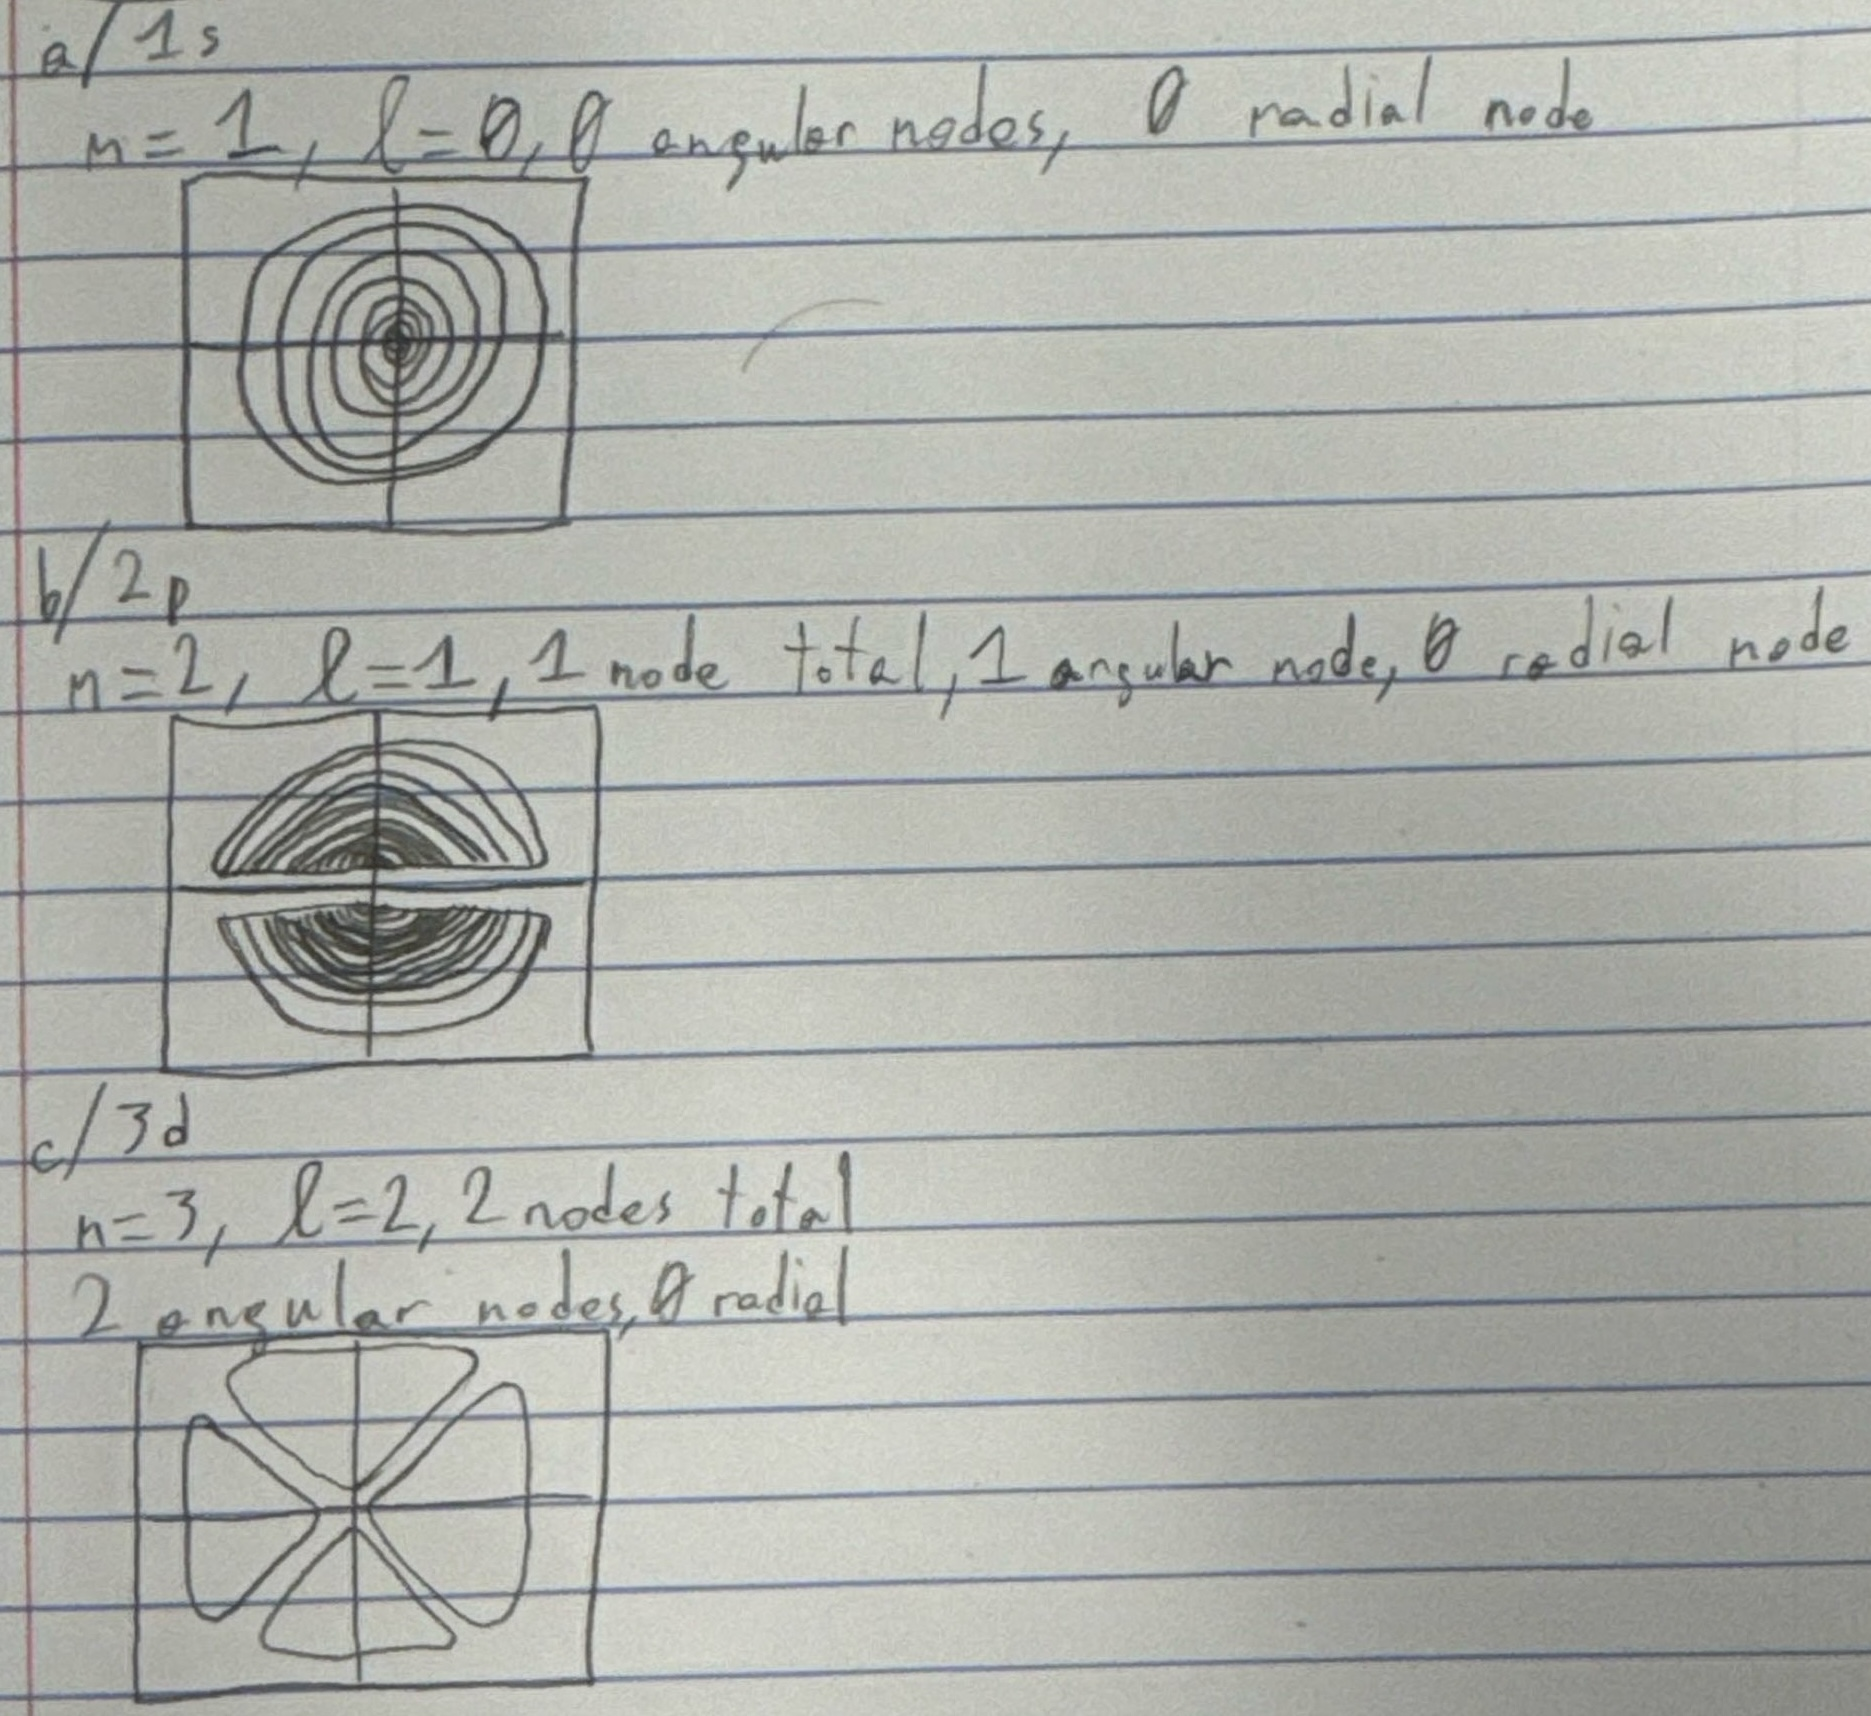
\includegraphics[width=\textwidth]{Answers Images/E21.jpg}
            \end{center}

    \pagebreak
    \section{Topic E Problem 21}
        \begin{enumerate}[label=\alph*)]
            \item   How does a 1s orbital differ from a 2s orbital?
            \item   How does a 2s orbital differ from a 2p orbital?
            \item   How does a 2p$_x$ orbital differ from a 2p$_y$ orbital?
            \item   How does a 3p orbital differ from a 4d orbital?
        \end{enumerate}
        
        \subsection{Solution (a)}
            A 2s orbital is of greater radius than a 1s orbital due to a higher energy.

        \subsection{Solution (b)}
            The shape is different.
            A 2p orbital would be two lobes along the x/y/z axis, while the 2s orbital would have a spherical orbital.

        \subsection{Solution (c)}
            The 2p$_x$ orbital's lobes would be centered around the x-axis, while the 2p$_y$ orbital's lobes would be centered around the y-axis.

        \subsection{Solution (d)}
            The 4d orbital would be bigger due to a higher energy, and it would also be have a different shape with more lobes. 

    \pagebreak
    \section{Topic E Problem 22}
        \begin{enumerate}[label=\alph*)]
            \item   How many different orbitals have n = 7? Explain your answer briefly.
            \item   How many different orbitals have n = 9 and $\ell$ = 7? Explain your answer briefly.
            \item   How many different orbitals have n = 8, $\ell$ = 5, and m$_\ell$ = -3? Explain your answer briefly.
            \item   How many different orbitals have n = 6 and m$_\ell$ = 2? Explain your answer briefly.
            \item   How many different orbitals have $\ell$ = 1 and m$_\ell$ = 0? Explain your answer briefly.
        \end{enumerate}
        
        \subsection{Solution (a)}
            For n = 7, $\ell$ has seven possible values: 0, 1, 2, and 3, 4, 5, and 6.
            For $\ell = 0$, there is 1 possible value of m$_\ell$.
            For $\ell = 1$, there is 3 possible values of m$_\ell$.
            For $\ell = 2$, there is 5 possible values of m$_\ell$.
            For $\ell = 3$, there is 7 possible values of m$_\ell$.
            For $\ell = 4$, there is 9 possible values of m$_\ell$.
            For $\ell = 5$, there is 11 possible values of m$_\ell$.
            For $\ell = 6$, there is 13 possible values of m$_\ell$.
            Adding these up, we get $1 + 3 + 5 + 7 + 9 + 11 + 13 = \boxed{49}$.
        
        \subsection{Solution (b)}
            For $\ell = 7$, there are \boxed{15} possible values of m$_\ell$, the number of integers between $-\ell$ and $\ell$, inclusive.
        
        \subsection{Solution (c)}
            In this case, all bases are covered in terms of atomic orbitals and there is no room for variation.
            As such, there is \boxed{1} orbital that fits this criteria.
        
        \subsection{Solution (d)}
            The varying value here is $\ell$.
            Having n = 6 sets an upper bound of the value of $\ell$ at 5.
            Meanwhile, having m$_\ell$ = 2 sets a lower bound of $\ell$ = 2.
            This gives \boxed{4} orbitals.
        
        \subsection{Solution (e)}
            Since there is no upper bound of $n$ dependant on either $\ell$ or m$_\ell$, there are an \U{infinite} number of orbitals that fit this.

    \pagebreak
    \tableofcontents
\end{document}